\documentclass[10pt,twocolumn,letterpaper]{article}

\usepackage{cvpr}
\usepackage{times}
\usepackage{epsfig}
\usepackage{graphicx}
\usepackage{amsmath}
\usepackage{amssymb}
\usepackage{comment}
\usepackage{booktabs,array}


% Include other packages here, before hyperref.

% If you comment hyperref and then uncomment it, you should delete
% egpaper.aux before re-running latex.  (Or just hit 'q' on the first latex
% run, let it finish, and you should be clear).
\usepackage[pagebackref=true,breaklinks=true,letterpaper=true,colorlinks,bookmarks=false]{hyperref}

\cvprfinalcopy % *** Uncomment this line for the final submission

\def\cvprPaperID{****} % *** Enter the CVPR Paper ID here
\def\httilde{\mbox{\tt\raisebox{-.5ex}{\symbol{126}}}}

% Pages are numbered in submission mode, and unnumbered in camera-ready
\ifcvprfinal\pagestyle{empty}\fi
\begin{document}

%%%%%%%%% TITLE
\title{Analysis of Dense Pixel Prediction Project Report : CS 7643}

\author{Yuemin Zhou, Brandon Sheffield, and Saheon Kim \\
Georgia Institute of Technology\\
{\tt\small \{yzhou43, bsheffield7, skim935\}@gatech.edu}
% For a paper whose authors are all at the same institution,
% omit the following lines up until the closing ``}''.
% Additional authors and addresses can be added with ``\and'',
% just like the second author.
% To save space, use either the email address or home page, not both
%\and
%Second Author\\
%Institution2\\
%First line of institution2 address\\
%{\tt\small secondauthor@i2.org}
}

\maketitle
%\thispagestyle{empty}

%%%%%%%%% ABSTRACT
\begin{abstract}
   In this group project report, we analyze dense pixel prediction performance such as object detection and semantic segmentation performance on a subset of the COCO 2017 dataset using limited computational resources. We distribute experiments among team members using distinct deep neural network architectures and collectively analyze the results. Future work proposes an architectural enhancement inspired by recent work done by Meta Research.
\end{abstract}

%%%%%%%%% BODY TEXT
\section{Introduction}

%(5 points) What did you try to do? What problem did you try to solve? Articulate your objectives using absolutely no jargon.

The underlying motivation behind this project for the team is to gain practical experience with handling 'large' datasets, modern deep neural network architectures, popular frameworks, and build up intuition through experimental results and analysis. The tasks we decided to focus on are common in dense prediction tasks\cite{vandenhende2021multi} found in computer vision such as object detection\cite{zaidi2022survey} and semantic segmentation\cite{lateef2019survey}. The object detection task involves identifying a particular class in an image and drawing a bounding box around it. The semantic segmentation task involves pixel level identification of similar objects as a single class.

To equally distribute contributions among the team, we each chose a deep neural architecture that is relevant to the tasks of object detection and semantic segmentation. Also a common framework is used among the team where each team member would have access to common building blocks, tools for analysis, and similar pipelines for training and testing models. This early decision would prove beneficial for assisting one another in troubleshooting and comparing methods. We leveraged the popular MMDetection\cite{mmdetection} toolbox. Further details on deep learning frameworks, existing code, source code for experiments, and models are detailed in the Appendix section \ref{existingCodeSection}.

For Faster RCNN, we want to test it on the truncated Coco 2017 dataset and see how compressed images effect the accuracy of the model. We will be using PCA to compress the images so there will be 3 datasets, one baseline and one that has 50 percent of the principle components and one that has 25 percent of the components. We will train the model on the baseline and compressed images and see how each model performs on the actual uncompressed images in test. We will also test pre-trained models and models with slight architectural differences on the same data set. 

%We want to analyze the performance of different architectures in the MMdetection model library against each other. They are specifically Faster RCNN, mask RCNN and Swin transformers. We also want to test the performance of some of these models with compressed images. 

%(5 points) How is it done today, and what are the limits of current practice?

%Faster RCNN as a baseline, Mask RCNN as an improvement and SWIN transformer as a further improvement? 

\subsection{Background}

The team ended up independently choosing two types of general neural network architectures, the Convolutional Neural Network(CNN) and the Visual Transformer(ViT). CNNs have seen an explosion of success in computer vision tasks in the last decade. CNNs are known to exhibit inductive biases that make them adept at analyzing images for examples. Such inductive biases include: locality, translation equivariance, and translation invariance. 

Currently many modern CNN's used in object detection add a feature pyramid network and a region proposal network on to the backbone CNN network. Faster RCNN is a form of this approach. The first layer is a CNN layer from resnet. It had four stages. The results of this layer are connected to a Feature Pyramid Network. The Feature Pyramid Network is a feature extractor which extracts the necessary feature maps that are needed for object detectors. At each stage of the resnet from the bottom up, a feature pyramid network will decrease spatial resolution and increase the semantic value. Therefore at the top layer the semantic value is highest. This top layer is then used to reconstruct layers or feature maps which are then used in the next step which is the region proposal network. 

In the region proposal network, first anchor points are generated. Every point in the feature map is an anchor point. Then anchor boxes are generated for every anchor point. These anchor boxes are generated with the scales and ratio set; they determine the sizes of the boxes. Initially these boxes are dummy boxes so the model has to learn whether the given box is foreground or background and at the same time it needs to learn the offsets to adjust the boxes so they fit the objects. This learning is done through regression. Once the foreground, background scores and offsets of anchor boxes are learned then the anchor boxes are processed again using proposal generation. Final proposals for the bounding box of an object are done through a region of interest pooling layer.



Inspired by the general learning architecture of transformers\cite{vaswani2017attention} that have made breakthroughs in natural language processing, vision transformers were introduced as a competitive architecture for computer vision tasks such as image classification\cite{dosovitskiy2020image} with reliance on large-scale pre-training data. There has been an explosion in transformer-based computer vision models with applications ranging from image retrieval\cite{el2021training}, object detection\cite{liu2021swin}, semantic segmentation\cite{wang2021pyramid}\cite{zhang2021multi}\cite{https://doi.org/10.48550/arxiv.2012.15840}, and video understanding\cite{https://doi.org/10.48550/arxiv.2103.15691}\cite{bertasius2021space}\cite{https://doi.org/10.48550/arxiv.2104.11227} have also shown promising results. Motivated by the success of visual transformers, self-supervised methods using vision transformers have been studied showing better results when self-training is applied as opposed to pre-training\cite{zoph2020rethinking}\cite{https://doi.org/10.48550/arxiv.2104.14294}.

However ViTs require vasts amount of data, time, and computational memory due to the quadratic cost of self-attention that is dependent on the number of patches. In object detection and segmentation tasks, a $wxh$ image has a complexity of $O(w^2h^2)$ when the images are high-resolution images. As a result, a general-purpose transformer backbone called the Swin Transformer\cite{liu2021swin} was proposed which constructs hierarchical feature maps and has linear computational complexity to image size. It inherits the advantages of the CNN as it fully considers the size invariance and relation between receptive fields. Limitations of the Swin Transformer is that it does not not have as many inductive biases as the CNN such as translation invariance. This in turns make learning very difficult requiring larger datasets and/or stronger data enhancements to achieve better learning performance.

\subsection{Motivation}

Object detection takes a lot of computational capacity and space. One area specifically is the images themselves; high quality images take up a lot of space. Therefore its worthwhile to explore methods that allow for a decrease in the space needed to store these images. We will decrease the quality of the images by taking smaller principle components of each image. This approach will simulate the use of lower quality images in training. 

Shortly after the introduction of the ViTs that showed to achieve comparable or even superior performance on image classification tasks, the Google Brain team analyzed how ViTs are solving these tasks and how do their learned representations compare to CNNs\cite{raghu2021vision}(inspired from the third graded discussion readings in this class). Their findings discovered that ViTs show strong preservation of spatial information which is useful in other computer vision tasks such as object detection. Since then, transformers have made their way into object detection setting key milestones\cite{arkin2021survey}:

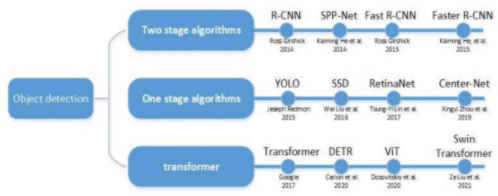
\includegraphics[width=0.8\linewidth]{docs/latex/images/brandon/ObjectDetection.png}
%\caption{Fig. 1 Object Detection algorithm milestones}

%(5 points) Who cares? If you are successful, what difference will it make?

The scope of our work is aimed at practitioners such as applied research scientists, machine learning engineers, robotics engineers, and anyone interested in practical performance of CNN and ViT based models perform. We motivate this project by diving deeper into the strengths and weaknesses of CNNs and ViTs through controlled experiments that compare performance on object detection and semantic segmentation tasks.

%%%%%%%%%%% DATASET
\subsection{Dataset}
%(5 points) What data did you use? Provide details about your data, specifically choose the most important aspects of your data mentioned \href{https://arxiv.org/abs/1803.09010}{here}. You don’t have to choose all of them, just the most relevant.

Here we briefly discuss the the most important aspects\cite{gebru2021datasheets} of the data used for experiments. We use the popular Microsoft COCO 2017 dataset\cite{lin2014microsoft} that commonly used to evaluate the performance of computer vision models. The name COCO standards for Common Objects in Context as it was designed to represent a vast array of everyday objects. It is widely considered the gold standard for tasks such as object detection, semantic segmentation, and key point detection. The data set consists of 121,408 images, 883, 331 object annotations, 80 classes, and an average image ratio of 640x480. For the experiments, we are interested in object detection and semantic segmentation performance.

Due to computational constraints and limitations of the models we chose we eventually settled on a truncated version of the COCO 2017 data set. This data set has the bbox annotations and the mask annotations needed for fast R-CNN and mask R-CNN. This data was further truncated to 1977 images for train, 500 for test, and 494 for validation. These images were all taken from the original training data set. This drastic truncation is needed due to our limited time and computational hardware.  

For the image compression experiments the images were converted to two compressed image sets. One set that has 50 percent of the principle components and another set that has 25 percent of the principle components. The training and validation data was converted this way but the test data was left the same to simulate how modeled trained on compressed images would perform in the real world. 

Also for coco we focused on one class classification because the classes in the dataset was quite imbalanced as can be seen from the following training class distribution figures:

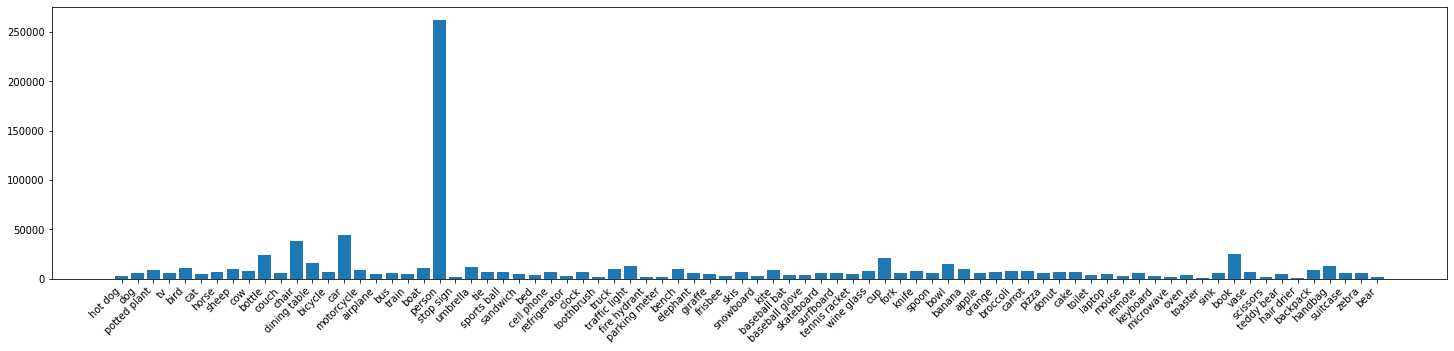
\includegraphics[width=0.8\linewidth]{docs/latex/images/brandon/coco17_train.png}
%\caption{Before: Training Class Distribution}

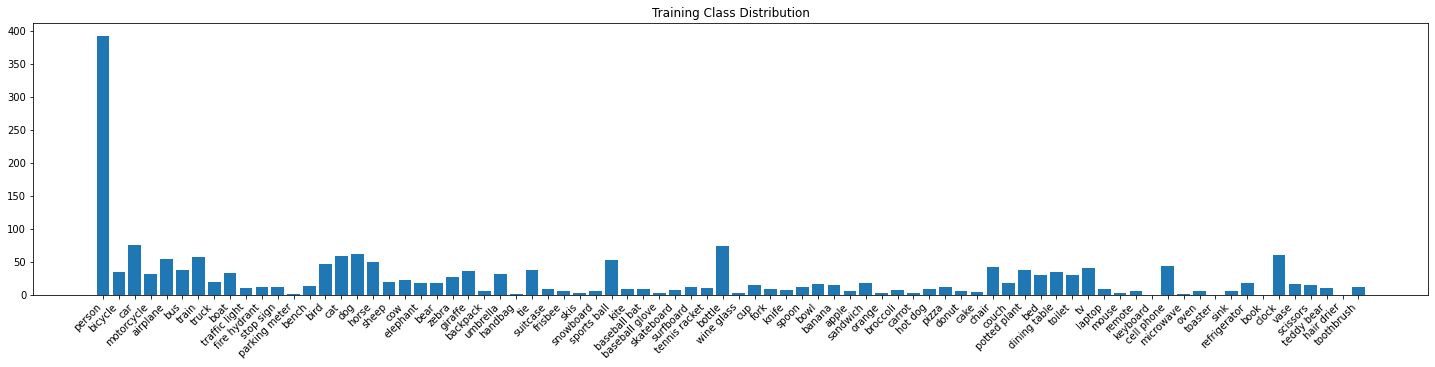
\includegraphics[width=0.8\linewidth]{docs/latex/images/brandon/coco17_train_trunc.png}
%\caption{After: Training Class Distribution}

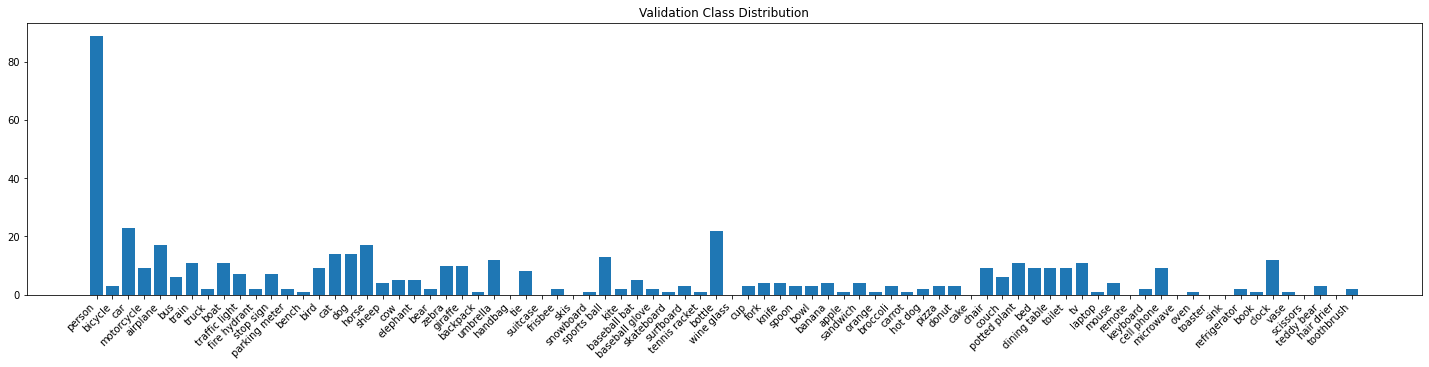
\includegraphics[width=0.8\linewidth]{docs/latex/images/brandon/coco17_val_trunc.png}
%\caption{After: Validation Class Distribution}

\section{Architecture Designs}



% Faster RCNN stuff moved to background. 

\subsubsection{Mask R-CNN Swin Transformer}


As illustrated in the following diagram, the deep neural network architecture presented is composed of 3 main components: backbone, neck, and model.

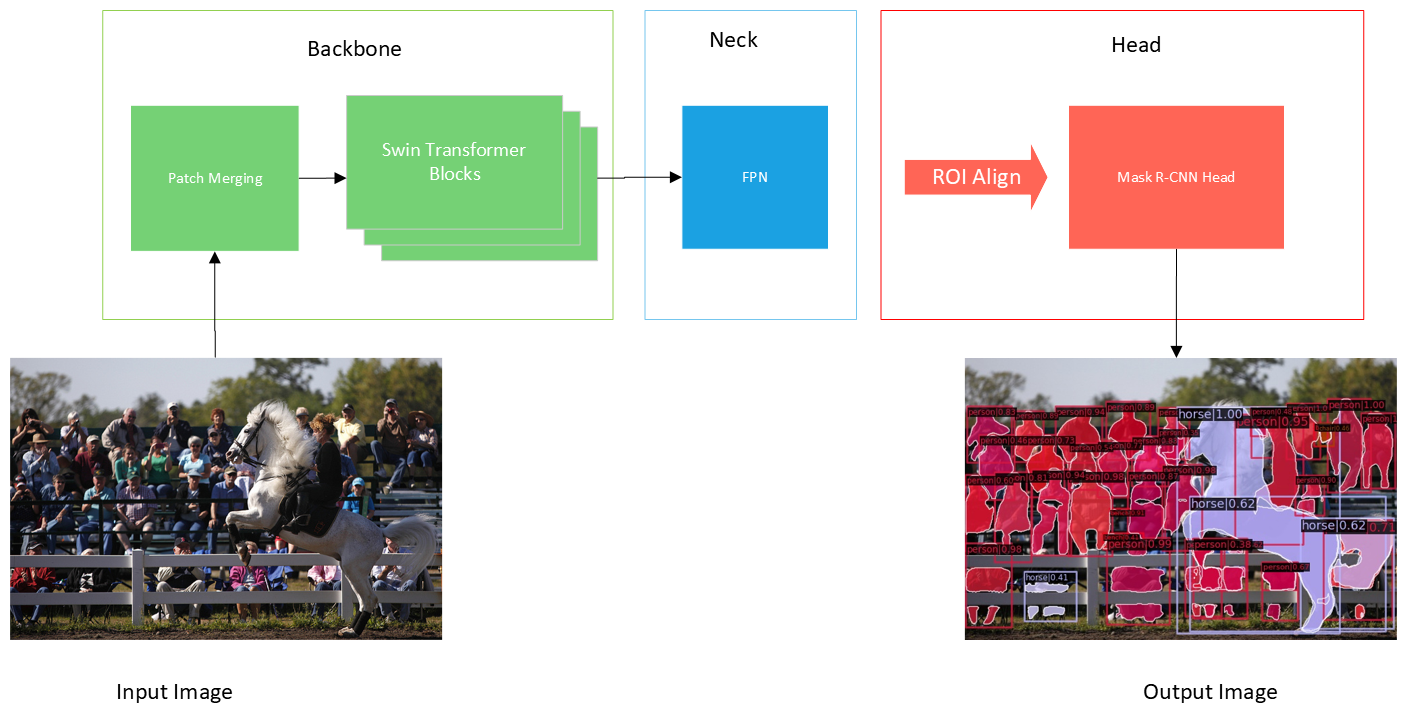
\includegraphics[width=1.0\linewidth]{docs/latex/images/brandon/Architecture.png}

Backbone - The Swin transformer builds a hierarchical transformer and performs self-attention calculations in the window area without overlap.

Neck - Feature Pyramid Network\cite{https://doi.org/10.48550/arxiv.1612.03144} is used as a feature extractor

Model - Mask-RCNN\cite{he2017mask} an extension of Faster R-CNN that has slightly more overhead that works by adding a branch for predicting an object mask called a Region of Interest (ROI) in parallel with an existing branch for recognition.

The train and test pipeline consists of a number of augmentations where the image is resized, randomly flipped, and normalized. The following is a table of hyper-parameters and values used.

%TODO brandon
%\subsection{Assessing the Loss}
%The Swin Transformer with Mask R-CNN uses cross entropy as it's loss function for assessing it's learning.
%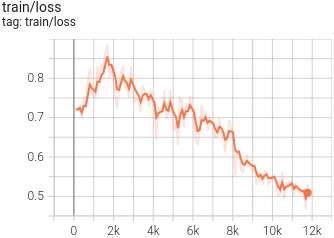
\includegraphics[width=0.8\linewidth]{docs/latex/images/brandon/Swin_train_loss.png}
%\caption{Swin Transformer Training Loss}

\begin{table}[htbp]
\centering
\caption{Highlighted Hyperparameters}
\label{table:hyper} 
\catcode`,=\active
\def,{\char`,\allowbreak}
\renewcommand\arraystretch{1.2}
\begin{tabular}{p{2.5cm}<{\raggedright} p{1cm} p{1cm}<{\raggedright} }
  \toprule
    Hyperparameters           & \textbf{Values} & \textbf{Selected Values}              \\ 
  \midrule
    Backbone                  & Window Size & 7                                   \\
    Optimizer                 & AdamW & 0.0001                                             \\ 
  \bottomrule
\end{tabular} 
\end{table}

The impact on the amount of data required to train effective transformers can be see with GradCam\cite{selvaraju2017grad}. Appendix \ref{SwinGradCamRefs} explores various Swin Transformer sizes trained on Imagenet1K and ImageNet21k datasets.

\subsubsection{RegNet Eric TODO}

%\begin{table}
%\begin{center}
%\begin{tabular}{|l|c|c|c|}
%\hline
%Backbone & Method   & Neck & Optimizer\\
%\hline\hline
%Swin-T   & Mask-RNN & FPN & AdamW\\
%\hline
%\end{tabular}
%\end{center}
%\caption{Deep Neural Architectures}
%\end{table}

%-------------------------------------------------------------------------
%------------------------------------------------------------------------
\section{Approach}

%(10 points) What did you do exactly? How did you solve the problem? Why did you think it would be successful? Is anything new in your approach?

The main objective we wanted to study was how well do the CNN and Transformer deep neural networks compare in controlled experiments on the same data set. We foresaw having different architectures being an issue when it came to comparing results and performance which motivated the idea of having a common framework. Upon doing research on object detection methods, we found a popular toolbox in which to base our experiments on, MMDetection\cite{mmdetection}. 

In the CNN model set we picked the Faster RCNN to do image compression experiments on. The compression experiments would be done on 3 different models; one without any pre-tuning, one with pre-tuning and one that has a slight architecture change and has no pre-tuning. The model that has the slight architecture change has the scales doubled from 8 to 16. Scales is one of the parameters that determine the anchor box sizes therefore we were hoping that large anchor boxes sizes could overcome the blurriness that comes with compressed images and therefore give better results. All three models will be trained and validated on three different data sets but will be tested on one data set. The three data sets used for training and validation are; a set of  uncompressed images, and a set of compressed images that have 50 percent principle components and a set of images that have only 25 percent principles components. All three data sets are the same truncated coco images and are essentially the same, other than the compression done by PCA. Testing data will only be on uncompressed images. Essentially we want to see how models perform on the original images when trained on compressed images.

For comparing models, CNN to transformers, we generated baseline performances on the truncated coco data set then did some fine-tuning of the model parameters. Existing pre-trained models were used as baselines. Fine tuning was done on model parameters and some architecture parameters as time allowed. An enhancement to the Swin Transformer is proposed in Appendix \ref{proposedSwin} that serves as future work.

%(5 points) What problems did you anticipate? What problems did you encounter? Did the very first thing you tried work?

The types of architectures that we experimented with and analyzed have an inherit difficulty in requiring lots of hardware resources such as storage and GPUs for training models from scratch. It was learned early that using the COCO 2017 dataset would involve several days of training as well as exceed current GPU resources which motivated the idea of reducing the dataset size. Even for training jobs such as fine-tuning, the authors experienced varying memory usages of 3GB to 10GB of GPU for small batch sizes which was surprising.

We also experiences issues with extracting certain metrics with mmdetection. Validation loss was one metric that we were not able to extract. In fact we found differences in results when calling a script to run the model vs running it extracting the functions from the files and running the model through those functions. We found that we can only get validation metrics, and even then it was only precision scores by running it from a script. This issue forced us to have to rerun everything to get some sort of validation metrics.   

%\textbf{Important: Mention any code repositories (with citations) or other sources that you used, and specifically what changes you made to them for your project. }

\subsection{Code and Model References}

See Appendix \ref{existingCodeSection}, regarding information related to deep learning frameworks, existing code, source code changes, and models used to produce experimental results.

\section{Experiments and Results}

%(10 points) How did you measure success? What experiments were used? What were the results, both quantitative and qualitative? Did you succeed? Did you fail? Why? Justify your reasons with arguments supported by evidence and data.

To measure success, we use common metrics found in object detection and semantic segmentation studies\cite{padilla2020survey} such as true positive(TP), false positive(FP), false negative(FN), precision(P), recall(R), Recall over Curve(ROC), intersection over union(IOU), mean average precision (mAP). All of these metrics compose the main ones we are interested in, namely box mAP and segmentation mAP, 

\begin{equation}
mAP = \frac{1}{N} \sum_{i=1}^N AP_i
\end{equation}

The following experiments evaluate model success through image compression performance, baseline mAP, fine-tuned mAP, overfitting, model complexity and performance where we also briefly introduce new metrics.

%\textbf{Important: This section should be rigorous and thorough. Present detailed information about decision you made, why you made them, and any evidence/experimentation to back them up. This is especially true if you leveraged existing architectures, pre-trained models, and code (i.e. do not just show results of fine-tuning a pre-trained model without any analysis, claims/evidence, and conclusions, as that tends to not make a strong project). }

\subsection{Faster RCNN Results for image compression}
These results are test data taken from a model that has the same baseline architecture but has not seen any pre-tuning or tuning. Faster RCNN does not have a Mask mAP component. 

\begin{table}[hbt!]
\begin{center}
\begin{tabular}{|l|c|}
\hline
Data used   & Box mAP \\
\hline\hline
uncompressed & 32.3 \\
compressed, 50 percent PCA used & 31.7 \\
compressed, 25 percent PCA used & 30.1 \\
\hline
\end{tabular}
\end{center}
\caption{Faster RCNN Baseline performance}
\end{table}

These results are test data taken from a model that has the same baseline architecture but has seen pre-tuning. Faster RCNN does not have a Mask mAP component. 

\begin{table}[hbt!]
\begin{center}
\begin{tabular}{|l|c|}
\hline
Data used   & Box mAP \\
\hline\hline
uncompressed & 54.6 \\
compressed, 50 percent PCA used & 54.5 \\
compressed, 25 percent PCA used & 53.0 \\
\hline
\end{tabular}
\end{center}
\caption{Faster RCNN pretuned performance}
\end{table}

These results are test data taken from a model that has a slight architecture adjustment which is doubling the scales used to generate the anchor boxes. The scales are used to generate the sizes of the anchor boxes; the idea is to increase them so that any blurriness from the compressed images can be overcome. No pre-tuning was done. 

\begin{table}[hbt!]
\begin{center}
\begin{tabular}{|l|c|}
\hline
Data used   & Box mAP \\
\hline\hline
uncompressed & 31.1 \\
compressed, 50 percent PCA used & 30.9 \\
compressed, 25 percent PCA used & 29.2 \\
\hline
\end{tabular}
\end{center}
\caption{Faster RCNN architecture adjustment performance}
\end{table}
\subsection{Baseline Results}

In order to gauge performance of experiments, we first established a baseline from pre-trained ImageNet-1K models. More specifically, we want to know the performance of the pre-trained ImageNet-1K model on it's ability to generalize to the truncated COCO 2017 dataset. One of the expectations we had for the experiment going in is that the pre-trained models would be able to generalize well in testing since there are common classes such as person. However, results were abysmal. We suspect the inherit difficulty bias in COCO coupled with overfitting of the ImageNet pre-trained models.


\begin{table}[hbt!]
\begin{center}
\begin{tabular}{|l|c|c|c|}
\hline
Backbone & Method   & Box mAP & Mask mAP \\
\hline\hline
Swin-T   & Mask-RNN & 0    & 0 \\
CNN   & Faster-RCNN & 0.1 & N/A \\
\hline
\end{tabular}
\end{center}
\caption{Baseline performance}
\end{table}

\subsection{Fine-Tuned Results}

TODO

\begin{table}[hbt!]
\begin{center}
\begin{tabular}{|l|c|c|c|}
\hline
Backbone & Method   & Box mAP & Mask mAP \\
\hline\hline
Swin-T   & Mask-RNN & 42.7    & 39.3 \\
\hline
\end{tabular}
\end{center}
\caption{Fine-tuned performance}
\end{table}

\subsection{Analysis of Results}

For the Faster RCNN experiments done on Image compression, the results showed that in all cases the models trained on uncompressed images did the best. However the 50 percent compressed image experiments did almost as good. Performance did seem to drop off much more when only 25 percent of the components are used. Therefore potentially we could train models on compressed images that only have 50 percent of the principle components and not get a large performance hit. 

Also the slight architecture change of doubling the scales did not result in better performance. This means that increasing the anchor box sizes did not result in better performance. Further analysis could be done with other parameters to change anchor box sizes however we did not have more time to do further experiments. 

\subsection{Overfitting and Generalization}

One of the problems we encountered is our inability to extract the validation losses from the training results. Therefore we had to look to other metrics to find if we are not over fitting and are generalizing well. One metric we looked at is training accuracy and the validation bbox average precision. We found that for all Faster RCNN cases both metrics are increasing therefore we can say that for the experiments on Faster RCNN we are not over-fitting. 

When exposed to new data in the validation set, the Swin Transformer is able to perform better overtime when measuring mAP bbox. Overfitting is not apparent.

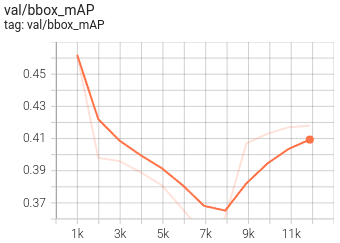
\includegraphics[width=0.8\linewidth]{docs/latex/images/brandon/swin_val_loss_bbox.png}
%\caption{Swin Transformer generalization}

\subsection{Model Performance and Complexity}

One of the constraints one has to consider when deploying a model into production is scalability. At max performance, how well does a model perform? Each model is evaluated on how many floating point operations required for a single forward pass measured in Floating Point Ops per Second (FLOPS). Higher values of FLOPS means the model is slower and has a lower throughput. The number of parameters, in millions (M), is also listed. This metric is useful for practitioners interested in models that can fit into low memory environments such as edge computing applications and robotics. Lastly we provide Frames Per Second (FPS) where each model is evaluated on how many images it can on average process of size 1280x720 pixels which is the common 720p standard high-definition display resolution.

\begin{table}[hbt!]
\begin{center}
\scalebox{0.9}{
\begin{tabular}{|l|c|c|c|c|}
\hline
Backbone & Method & FLOPS (G) & Params (M) & FPS \\
\hline\hline
Swin-T   & Mask-RNN & 263 & 48 & 23.8 \\
CNN   & Faster-RCNN & 202 & 41 & 15.4 \\
\hline
\end{tabular}
}
\end{center}
\caption{Model performance and complexity with 720p images}
\end{table}

As one can see, there is a performance gap between the Swin-T Mask-RNN and Faster-RCNN model. There appears to be a correlation between FLOPS and number of parameters. This makes sense intuitively that a larger complex model implies that there are more floating operations to perform. What is surprising is that the Swin-T model is able to process more images per second than the Faster-RCNN model.

\section{Experiences}

\subsection{Challenges}

We first proposed a group project on detecting 3D objects from point cloud data. It was obvious to us that the topic was a hot research area with the motivation of self-driving applications at the wheel. However, once the team became hands-on with the point cloud data, it became apparent that interprability and specialized tools required to interpret sparse point cloud data was not as natural as typical camera images. We then changed topics to more relatable material covered in class such as CNNs and transforms from NLP while staying consistent with object detection.

Finding the right dataset was also a challenge. Initially we picked the kitti dataset because it's data was focused on autonomous driving and have viewpoints from the car. Also it seemed compatible with Faster RCNN. However we later found that it did not have the annotations needed for Swin implementation and we had to pivot. 

\subsection{New Challenges}

Whether processing point cloud data or camera images with recent methods, computational resources such as access to enterprise GPUs would always prove to be a challenge. Training on large datasets requires large batch sizes affecting training time and model performance.

\subsection{Team Achievements}

Although the computational resources were out of reach for the team using Colab and local GPU resources, we effectively learned about bleeding edge research topics in computer vision that are actively being improved and published on. We were able to do sensitivity studies on compressed images and do some trials and experimentation's with some of the most advanced methods currently in use. For example, ViTs have a new workshop at CVPR 2022 since their introduction in 2020. Also the Swin Transformer won the ICCV 2021 best paper award. There has also been a published Swin Transformer v2 and complementary SimMIM that have been accepted for ICCV 2022. We see this exposure as an advantage for collaboration and future work with prospective research teams from the private and public sectors.


%-------------------------------------------------------------------------
%\section{Other Sections}

%You are welcome to introduce additional sections or subsections, if required, to address the following questions in detail. 

%(5 points) Appropriate use of figures / tables / visualizations. Are the ideas presented with appropriate illustration? Are the results presented clearly; are the important differences illustrated? 

%(5 points) Overall clarity. Is the manuscript self-contained? Can a peer who has also taken Deep Learning understand all of the points addressed above? Is sufficient detail provided? 

%(5 points) Finally, points will be distributed based on your understanding of how your project relates to Deep Learning. Here are some questions to think about: 

%What was the structure of your problem? How did the structure of your model reflect the structure of your problem? 

%What parts of your model had learned parameters (e.g., convolution layers) and what parts did not (e.g., post-processing classifier probabilities into decisions)? 

%What representations of input and output did the neural network expect? How was the data pre/post-processed?

%What was the loss function? 

%Did the model overfit? How well did the approach generalize? 

%What hyperparameters did the model have? How were they chosen? How did they affect performance? What optimizer was used? 

%What Deep Learning framework did you use? 

%What existing code or models did you start with and what did those starting points provide? 

%Note that at least some of these questions and others should be relevant to your project and should be addressed in the PDF. You do not need to address all of them in full detail. Some may be irrelevant to your project and others may be standard and thus require only a brief mention. For example, it is sufficient to simply mention the cross-entropy loss was used and not provide a full description of what that is. Generally, provide enough detail such that someone with an appropriate background (in both Deep Learning and your domain of choice) could replicate the main parts of your project somewhat accurately. 

%-------------------------------------------------------------------------
\section{Future Work}

An on-going debate in neural architecture design revolves around balancing width and depth. The first successful neural networks on Imagenet were considered deep in 2014 standards\cite{krizhevsky2012imagenet}\cite{simonyan2014very}. With the introduction of ResNets\cite{he2016deep}\cite{he2016identity} optimization with deep layers suffered due to the residual connections. This deep optimization problem motivated researchers to analyze the trade-offs associated with depth and width\cite{ding2021repvgg}\cite{huang2016deep}\cite{zagoruyko2016wide}. 

There are a number of published works interested in shallower neural networks\cite{goyal2021non}\cite{zagoruyko2016wide} for reasons such as lower latency to easier optimization. One of the simple proposed methods advocates parallel vision transformers\cite{touvron2022three} that takes a sequential architecture and reorganizes the blocks by pairs. The overall result is an architecture that is wider and shallower which is an effective design for more parallel processing, easing optimization, and the reduction of latency dependent on the implementation.

With the rise of attention-based neural networks, wider architectures is once again being revisited\cite{goyal2021non}. In the work "Non-deep Networks", an architecture with several parallel branches is proposed that leads to more complex design. In the work, "Three things everyone should know about Vision Transformers", the authors propose three methods for ViTs that are much simpler and flexible alternative methods: parallel blocks, fine-tuning, patch pre-processing\cite{touvron2022three}.

Future work motivated by the implementation of these three methods mechanisms into the Swin Transformer shows promise. In the appendix section \ref{proposedSwin}, it is illustrated how the parallel blocks can be implemented for future research opportunities.

%-------------------------------------------------------------------------

\section{Work Division}
%TODO this freaking table will not go where it is expected.

\begin{table}[h!]
\begin{center}
\scalebox{1.0}{
\begin{tabular}{|l|c|}
\hline
Student Name & Impl/Experiments/Analysis \\
\hline\hline
Yuemin Zhou & Faster R-CNN   \\
Brandon Sheffield & Swin Transformer  \\
Saheon Kim & Mask R-CNN  \\
\hline
\end{tabular}
}%scalebox
\end{center}
\caption{Contributions of team members.}
\label{tab:contributions}
\end{table}

%References
{\small
\bibliographystyle{ieee_fullname}
\bibliography{egbib}
}

\clearpage
\appendix
\label{sec:appendix}

\section{Existing Code and Models} \label{existingCodeSection}


\begin{table}[h!]
\begin{center}
\begin{tabular}{||c|c||}
\hline
References & Online Sources \\
\hline\hline
Deep Learning Framework & https://pytorch.org/ \\
Detection Framework     & https://github.com/open-mmlab/mmdetection \\
Brandon Sheffield       & https://github.com/mastash3ff/cs7643-GroupProject \\
Swin Transformer Models & https://github.com/open-mmlab/mmdetection/tree/master/configs/swin \\
ViT Gradcam & https://github.com/jacobgil/pytorch-grad-cam \\
\hline
\end{tabular}
\end{center}
\label{tab:existing}
\end{table}

\clearpage

\section{Proposed Swin Transformer Enhancement} \label{proposedSwin}

%%%%%%%%%%%%%%%%%%%%%%%%%%%%%%%%%%%%%%%%%%%%%%%%%%%%%%%%%%%%%%%%

%Since the introduction of the Swin Transformer in 2020, there has been improvements in regards to scaling up it's capacity and resolution\cite{liu2021swinV2}. Additionally, there have been self-supervised learn methods proposed such as MoBY\cite{xie2021moby} which combines MoCo\cite{he2020momentum}\cite{chen2020improved} with BYOL\cite{grill2020bootstrap} and SimMIM\cite{xie2021simmim} where they use the Swin Transformer backbone.

An enhancement that is proposed for the Swin Transformer is the use of parallel blocks that results in an architecture that has the same number of parameters and computational complexity while being wider and shallower. This insight was realized while surveying ViTs\cite{touvron2022three} and realized not to exist in Swin Transformer implementations as far as we know.

Given a sequence of transformer blocks:

\begin{equation}
x^{'}_{i+1} = x_1 + mhsa_l(x_l)
\end{equation}

\begin{equation}
x^{'}_{i+1} = x^{'}_{1+1} + ffn_l(x^{'}_{l+1})
\end{equation}

\begin{equation}
x^{'}_{i+2} = x_{1+1} + mhsa_{l+1}(x_{l+1})
\end{equation}

\begin{equation}
x_{i+2} = x^{'}_{1+2} + mhsa_{l+1}(x^{'}_{l+2})
\end{equation}

these transformer blocks are combined into two parallel operations:

\begin{equation}
x_{l+1} = x_{l} + mhsa_{l,1}(x_l) + mhsa_{l,2}(x_l)
\end{equation}

\begin{equation}
x_{l+2} = x_{l+1} + ffn_{l,1}(x_l+1) + ffn_{l,2}(x_{l+1})
\end{equation}


The two parallel operations effectively result in twice the amount of processing that is performed in parallel while reducing the number of layers by two.

Here we illustrate the sequential then proposed parallel block methods for ViTs. Given a sequence of transformer blocks:

\begin{equation}
x^{'}_{i+1} = x_1 + mhsa_l(x_l)
\end{equation}

\begin{equation}
x^{'}_{i+1} = x^{'}_{1+1} + ffn_l(x^{'}_{l+1})
\end{equation}

\begin{equation}
x^{'}_{i+2} = x_{1+1} + mhsa_{l+1}(x_{l+1})
\end{equation}

\begin{equation}
x_{i+2} = x^{'}_{1+2} + mhsa_{l+1}(x^{'}_{l+2})
\end{equation}

The original authors proposed the following parallel transformer blocks:

\begin{equation}
x_{l+1} = x_{l} + mhsa_{l,1}(x_l) + mhsa_{l,2}(x_l)
\end{equation}

\begin{equation}
x_{l+2} = x_{l+1} + ffn_{l,1}(x_l+1) + ffn_{l,2}(x_{l+1})
\end{equation}

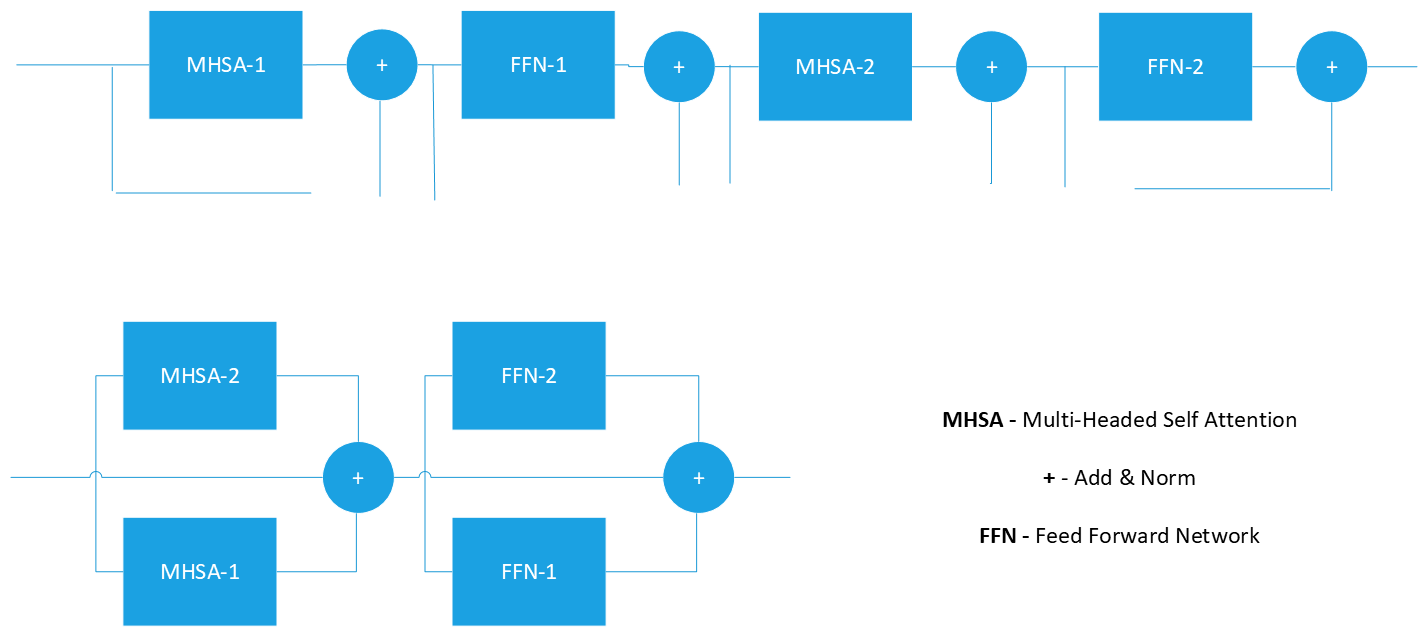
\includegraphics[width=0.8\linewidth]{docs/latex/images/brandon/MHSA-Original.png}
%\caption{Top - Original sequential attention blocks. Bottom - parallel attention blocks.}

The Swin Transformer is notably a variant of the original ViT therefore there are design changes to consider. For one, the Swin Transformer introduces the ideas of using the regular and shifted windows for computing attention which is not found in classic ViTs. The use of these windows avoids quadratic complexity of global attention with respect to the number of tokens as it would require an intractable amount of tokens for dense prediction tasks as well as computing on high-resolution images. The equations for computing these two windows are as followed:

\begin{equation}
\omega(MSA) = 4hwC^2 + 2(hw)^2C,
\end{equation}

\begin{equation}
\omega(W-MSA) = 4hwC^2 + 2M^2hwC,
\end{equation}

These windows can now be placed into the Swin Transformer blocks:

\begin{equation}
z^{l} = W-MSA (LN(z^{l-1})) + z^{l-1}
\end{equation}

\begin{equation}
z^{l} = MLP (LN(z^{l})) + z^{l}
\end{equation}

\begin{equation}
z^{l+1} = W-MSA (LN(z^{l-1})) + z^{l-1}
\end{equation}

\begin{equation}
z^{l+1} = MLP (LN(z^{l+1})) + z^{l+1}
\end{equation}

The insight of parallel blocks can be adapted to Swin Transformers\cite{liu2021swin} which is a variant of ViTs. The original Swin Transformer two block layout is defined as:

\begin{equation}
x^{'}_{i+1} = x_1 + mhsa_l(x_l)
\end{equation}

\begin{equation}
x^{'}_{i+1} = x^{'}_{1+1} + ffn_l(x^{'}_{l+1})
\end{equation}

\begin{equation}
x^{'}_{i+2} = x_{1+1} + mhsa_{l+1}(x_{l+1})
\end{equation}

\begin{equation}
x_{i+2} = x^{'}_{1+2} + mhsa_{l+1}(x^{'}_{l+2})
\end{equation}

It can be observed that these two Swin Transformer blocks can also be placed in parallel fashion.

\begin{equation}
x_{l+1} = x_{l} + mhsa_{l,1}(x_l) + mhsa_{l,2}(x_l)
\end{equation}

\begin{equation}
x_{l+2} = x_{l+1} + ffn_{l,1}(x_l+1) + ffn_{l,2}(x_{l+1})
\end{equation}

%\caption{Swin Transformer Parallel Blocks}
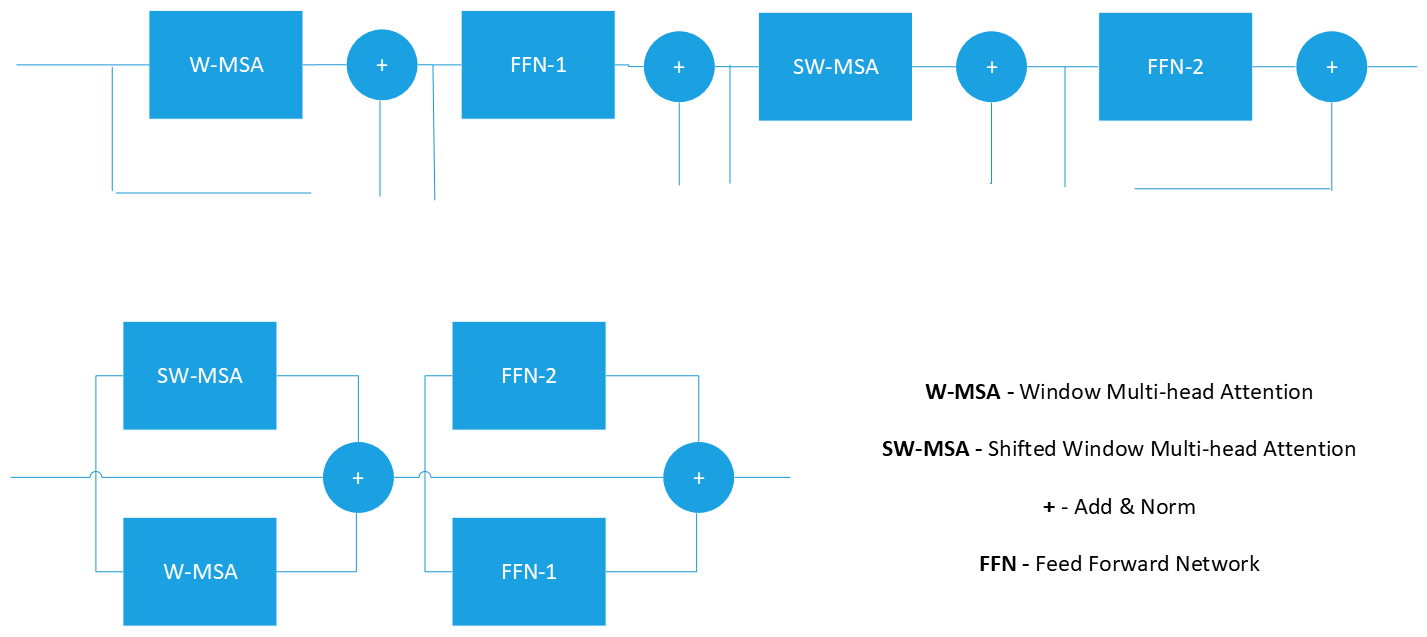
\includegraphics[width=0.8\linewidth]{docs/latex/images/brandon/MSA-Swin.png}
%\caption{}
%\end{comment}
\clearpage

\section{Swin Gradcam} \label{SwinGradCamRefs}

Visual Transformers are sensitive to the amount of data used to train them. This can be seen when the size of the models grow. The gradients can be visualized of where the network pays the most attention to in the following series of images.

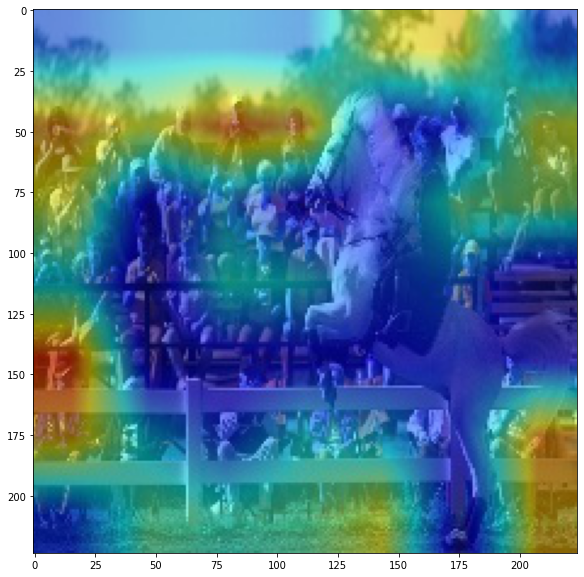
\includegraphics[width=0.8\linewidth]{docs/latex/images/brandon/gradcam_tiny_swin.png}
%\caption{GradCam Swin Transformer Tiny trained on ImageNet1K}

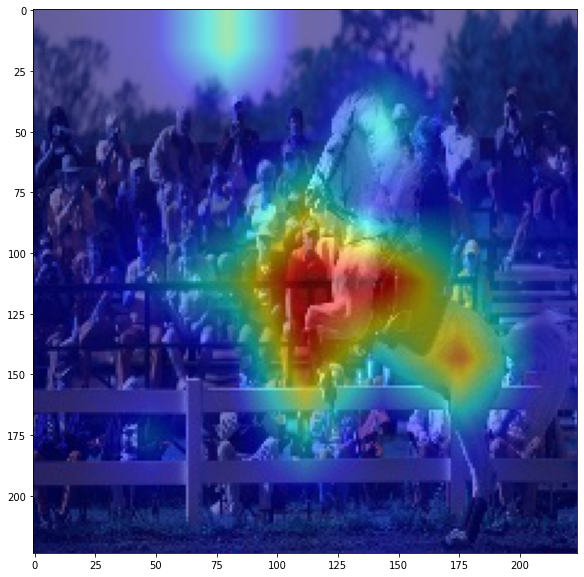
\includegraphics[width=0.8\linewidth]{docs/latex/images/brandon/gradcam_base_swin.png}
%\caption{GradCam Swin Transformer Base trained on ImageNet1K}

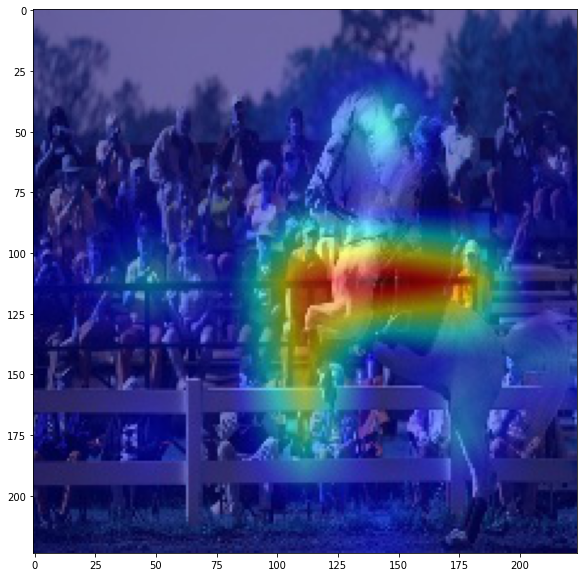
\includegraphics[width=0.8\linewidth]{docs/latex/images/brandon/gradcam_large_swin_patch4_window7_224_in22k.png}
%\caption{Gradcam Swin Transformer Large trained on ImageNet22K}



\end{document}

